\documentclass[letterpaper]{article}
\usepackage{aaai24}
\usepackage{times}
\usepackage{helvet}
\usepackage{courier}
\usepackage[hyphens]{url}
\usepackage{graphicx}
\graphicspath{{figures/}}
\urlstyle{rm}
\usepackage{amsmath}
\usepackage{amssymb}
\usepackage{booktabs}
\usepackage{algorithm}
\usepackage{algorithmic}
\usepackage{natbib}
\usepackage{float}

\frenchspacing
\setlength{\pdfpagewidth}{8.5in}
\setlength{\pdfpageheight}{11in}

\title{Homework 2: Q-Learning for Parking Lot Navigation\\Question Responses}
\author{
    Josh Manchester\\
    Department of Computer Science\\
    University of Colorado Colorado Springs\\
    Colorado Springs, CO 80918\\
    \texttt{jmanches@uccs.edu}
}

\begin{document}
\maketitle

\section{Problem 1: Tabular Q-Learning}

\subsection{Problem 1a: Environment Representation}

The parking lot is modeled as a $7 \times 6$ grid (7 rows, 6 columns) matching the layout in Figure~1 of the assignment. The agent starts at the entrance at position $(6, 5)$ and must navigate to one of 8 parking spots. BFS verification confirms optimal paths range from 3 steps (P8, nearest) to 10 steps (P1, farthest).

\textbf{State space.} A state is a tuple $(r, c, g)$ where $(r, c)$ is the car's row and column position and $g \in \{0, \ldots, 7\}$ identifies the target parking spot. The goal is part of the state because the walkable cells change depending on which spot is the target---non-target parking spots act as walls that the car cannot drive over. This means each goal creates a different navigation problem with its own set of reachable cells.

\textbf{Action space.} Four discrete actions: UP (row $-1$), DOWN (row $+1$), LEFT (col $-1$), RIGHT (col $+1$). There is no angular steering---the car moves one cell per step in one of the four cardinal directions.

\textbf{Reward structure.} The reward function uses three values:
\begin{itemize}
    \item $+10.0$ for reaching the goal parking spot (episode terminates)
    \item $-0.1$ per valid step (encourages the shortest path)
    \item $-1.0$ for hitting a wall, barrier, or grid edge (agent stays in place)
\end{itemize}
The step penalty pushes the agent toward the BFS-optimal path. The wall penalty discourages the agent from repeatedly bumping into obstacles. The large positive terminal reward makes reaching the goal clearly preferable to wandering.

\textbf{Barrier modeling.} Row 3, columns 1 through 4 are barrier cells. Any action that would move the agent into a barrier cell is treated identically to hitting the grid boundary---the agent stays where it is and receives the $-1.0$ wall penalty. Columns 0 and 5 of row 3 are open driving lanes, providing passages on both sides of the barrier.

\textbf{Edge handling.} Before executing a move, the environment checks whether the resulting position $(r', c')$ satisfies $0 \le r' < 7$ and $0 \le c' < 6$. If the move would take the agent out of bounds, the agent stays in place and receives the $-1.0$ penalty. The same check applies to barrier cells and non-target parking spots.

\textbf{Q-table structure.} The Q-table is implemented as a Python dictionary mapping $(r, c, g, a) \to \mathbb{R}$, where $a \in \{0, 1, 2, 3\}$ is the action index. All entries are initialized to 0. Using a dictionary rather than a dense array avoids allocating memory for state-action pairs that are never visited (barrier cells, out-of-bounds states). For the $7 \times 6$ grid with 8 goals and 4 actions, the maximum table size is $7 \times 6 \times 8 \times 4 = 1{,}344$ entries, though in practice only the reachable states are populated during training.

\textbf{Reachability verification.} Before training begins, BFS is run from the entrance to every parking spot to confirm all 8 goals are reachable. This catches layout errors early. The BFS shortest path lengths also serve as the ground truth for evaluating whether the learned policies are optimal.

\subsection{Problem 1b: Q-Learning and Double Q-Learning Algorithms}

\subsubsection{Q-Learning}

Algorithm~\ref{alg:qlearning} presents the tabular Q-learning algorithm with $\varepsilon$-greedy exploration.

\begin{algorithm}[t]
\caption{Q-Learning with $\varepsilon$-Greedy Exploration}
\label{alg:qlearning}
\begin{algorithmic}[1]
\STATE Initialize $Q(s, a) = 0$ for all $s \in \mathcal{S}, a \in \mathcal{A}$
\STATE Set $\alpha = 0.1$, $\gamma = 0.99$, $\varepsilon = 1.0$, $\varepsilon_{\min} = 0.01$, $\varepsilon_{\text{decay}} = 0.995$
\FOR{each episode $= 1, 2, \ldots, N$}
    \STATE Sample goal $g$ uniformly from $\{0, \ldots, 7\}$
    \STATE $S \leftarrow$ entrance position $(6, 5)$
    \WHILE{$S$ is not terminal \AND steps $<$ max\_steps}
        \IF{random() $< \varepsilon$}
            \STATE $A \leftarrow$ random action \hfill \textit{// explore}
        \ELSE
            \STATE $A \leftarrow \arg\max_a Q(S, a)$ \hfill \textit{// exploit}
        \ENDIF
        \STATE Take action $A$, observe reward $R$ and next state $S'$
        \IF{$S'$ is terminal}
            \STATE $Q(S, A) \leftarrow Q(S, A) + \alpha \left[ R - Q(S, A) \right]$
        \ELSE
            \STATE $Q(S, A) \leftarrow Q(S, A) + \alpha \left[ R + \gamma \max_{a'} Q(S', a') - Q(S, A) \right]$
        \ENDIF
        \STATE $S \leftarrow S'$
    \ENDWHILE
    \STATE $\varepsilon \leftarrow \max(\varepsilon_{\min},\ \varepsilon \cdot \varepsilon_{\text{decay}})$
\ENDFOR
\end{algorithmic}
\end{algorithm}

Line 1 initializes the Q-table optimistically at zero. Since most transitions yield negative rewards ($-0.1$ or $-1.0$), zero initialization encourages exploration of unvisited states.

Lines 7--11 implement $\varepsilon$-greedy action selection. Early in training, $\varepsilon \approx 1.0$, so the agent explores randomly. As $\varepsilon$ decays (line 19), the agent increasingly exploits the learned Q-values.

Lines 14--16 are the core Q-learning update. The key term is $\max_{a'} Q(S', a')$---Q-learning bootstraps from the \textit{best possible} next action regardless of which action was actually taken. This makes Q-learning an \textit{off-policy} algorithm: it learns about the greedy policy while following an exploratory policy.

Line 19 decays $\varepsilon$ after each episode. The decay factor of 0.995 means $\varepsilon$ reaches approximately 0.01 after 920 episodes, at which point the agent is mostly greedy with occasional random exploration.

\subsubsection{Double Q-Learning}

Algorithm~\ref{alg:doubleq} presents the Double Q-learning variant.

\begin{algorithm}[t]
\caption{Double Q-Learning}
\label{alg:doubleq}
\begin{algorithmic}[1]
\STATE Initialize $Q_1(s, a) = 0$ and $Q_2(s, a) = 0$ for all $s, a$
\STATE Set $\alpha$, $\gamma$, $\varepsilon$, $\varepsilon_{\min}$, $\varepsilon_{\text{decay}}$
\FOR{each episode}
    \STATE Sample goal $g$, set $S \leftarrow$ entrance
    \WHILE{$S$ is not terminal \AND steps $<$ max\_steps}
        \STATE Choose $A$ via $\varepsilon$-greedy using $\frac{Q_1(S,\cdot) + Q_2(S,\cdot)}{2}$
        \STATE Take action $A$, observe $R$, $S'$
        \IF{random() $< 0.5$}
            \STATE $A^* \leftarrow \arg\max_a Q_1(S', a)$ \hfill \textit{// Q1 selects}
            \STATE $Q_1(S,A) \leftarrow Q_1(S,A) + \alpha[R + \gamma\, Q_2(S', A^*) - Q_1(S,A)]$ \hfill \textit{// Q2 evaluates}
        \ELSE
            \STATE $A^* \leftarrow \arg\max_a Q_2(S', a)$ \hfill \textit{// Q2 selects}
            \STATE $Q_2(S,A) \leftarrow Q_2(S,A) + \alpha[R + \gamma\, Q_1(S', A^*) - Q_2(S,A)]$ \hfill \textit{// Q1 evaluates}
        \ENDIF
        \STATE $S \leftarrow S'$
    \ENDWHILE
    \STATE Decay $\varepsilon$
\ENDFOR
\end{algorithmic}
\end{algorithm}

\textbf{How Double Q-Learning improves on Q-Learning.} Standard Q-learning suffers from \textit{maximization bias}. The $\max_{a'} Q(S', a')$ term in the update uses the same Q-values both to select the best action and to estimate its value. When Q-values contain noise (which they always do during learning), taking the maximum over noisy estimates systematically overestimates the true value \citep{hasselt2010double}.

Double Q-learning fixes this by maintaining two independent Q-tables. On each update step, one table selects the best action (line 9 or 12) while the other evaluates it (line 10 or 13). This decoupling breaks the positive bias because the noise in the selecting table is independent of the noise in the evaluating table.

For action selection during episodes (line 6), the agent uses the average of both tables, which provides a more stable estimate than either table alone.

Empirically, standard Q-learning's mean max Q-values are consistently higher than Double Q-learning's throughout training, confirming the overestimation. In our deterministic environment this bias does not affect the final policy (both algorithms find optimal paths), but in stochastic environments it can lead to suboptimal action selection.


\section{Problem 2: Deep Q-Learning}

\subsection{Problem 2a: Neural Network Design}

\textbf{Inputs.} The neural network receives a 4-dimensional vector:
\begin{equation}
    \mathbf{x} = \left[\frac{r}{6},\ \frac{c}{5},\ \frac{g_r}{6},\ \frac{g_c}{5}\right]
\end{equation}
where $(r, c)$ is the car's position and $(g_r, g_c)$ is the goal parking spot's position. All values are normalized to $[0, 1]$ by dividing by the maximum row index (6) and column index (5). The goal position is included as input so a single network can learn policies for all 8 parking spots simultaneously.

\textbf{Outputs.} The network outputs 4 Q-values, one for each action (UP, DOWN, LEFT, RIGHT). The agent selects the action with the highest Q-value (during greedy execution) or a random action with probability $\varepsilon$ (during training).

\textbf{What the network learns.} The network learns the function $Q(s, a; \theta) \approx Q^*(s, a)$---the optimal action-value function. Given a state-goal encoding, it predicts the expected discounted return for each action. Once trained, the greedy policy $\pi(s) = \arg\max_a Q(s, a; \theta)$ should match the optimal BFS policy.

\textbf{Architecture.} The network is a fully connected feedforward network with two hidden layers:
\[
    \text{Input}(4) \to \text{FC}(128) \to \text{ReLU} \to \text{FC}(128) \to \text{ReLU} \to \text{FC}(4)
\]
This architecture was chosen for several reasons. Two hidden layers provide enough capacity to learn the non-linear mapping from positions to Q-values without being so deep that training becomes unstable. The 128-unit width was determined empirically---64 units were insufficient for consistent convergence across all 8 goals, while 128 units achieved 100\% success. ReLU activations are standard for DQN and avoid vanishing gradient issues. The total parameter count is approximately 17,540.

\textbf{Replay memory.} A circular buffer (Python \texttt{deque}) stores transitions as named tuples $(s, a, r, s', \text{done})$ where $s$ and $s'$ are the 4-dimensional encoded vectors. The buffer has a capacity of 20,000 transitions. When full, new transitions overwrite the oldest ones.

The buffer is filled online during training: every time the agent takes a step in the environment, the resulting transition is pushed into the buffer. Training begins once 64 transitions have accumulated (one full batch). On every subsequent step, a random mini-batch of 64 transitions is sampled from the buffer for one gradient update.

\textbf{Why replay memory?} Without replay, consecutive training samples are highly correlated (adjacent states in the same episode). This correlation destabilizes neural network training because gradient updates on correlated samples reinforce each other, causing the network to overfit to recent experience and forget earlier lessons. Random sampling from the buffer breaks these correlations, providing the i.i.d.-like samples that gradient descent assumes \citep{mnih2015human}.

\textbf{Buffer size considerations.} A buffer of 20,000 transitions holds roughly the last 2,000--3,000 episodes of experience (at an average of 7 steps per episode once the agent is proficient). This is large enough to decorrelate samples while small enough to keep the data relevant---too large a buffer fills with low-quality early-exploration transitions that slow convergence. We tested sizes from 1,000 to 50,000 and found that 10,000--20,000 provided the best balance.

\textbf{Target network.} A copy of the Q-network (the ``target network'') provides stable TD targets during training. It is updated every 50 episodes by copying the weights from the online network. Without the target network, the TD target $r + \gamma \max_{a'} Q(s', a'; \theta)$ shifts with every gradient step, creating a moving target that can cause training divergence.

\textbf{Training details.} Adam optimizer, learning rate $5 \times 10^{-4}$, MSE loss, batch size 64. Exploration uses $\varepsilon$-greedy with decay factor 0.998 (slower than tabular, because neural convergence benefits from extended exploration). Training runs for 15,000 episodes on the base $7 \times 6$ grid.


\subsection{Problem 2b: Results and Parameter Sensitivity}

\textbf{Learned policies.} All three algorithms (Q-learning, Double Q-learning, DQN) achieve 100\% success rates across all 8 parking spots. The learned path lengths match the BFS-optimal paths exactly. Table~\ref{tab:results} shows the evaluation results.

\begin{table}[H]
\centering
\caption{Evaluation results (100 episodes per goal, all three algorithms)}
\label{tab:results}
\begin{tabular}{@{}ccccc@{}}
\toprule
Spot & Success & Avg Steps & Avg Reward & BFS Optimal \\
\midrule
P1 & 100\% & 10.0 & 9.10 & 10 \\
P2 & 100\% & 9.0  & 9.20 & 9 \\
P3 & 100\% & 8.0  & 9.30 & 8 \\
P4 & 100\% & 5.0  & 9.60 & 5 \\
P5 & 100\% & 6.0  & 9.50 & 6 \\
P6 & 100\% & 5.0  & 9.60 & 5 \\
P7 & 100\% & 4.0  & 9.70 & 4 \\
P8 & 100\% & 3.0  & 9.80 & 3 \\
\bottomrule
\end{tabular}
\end{table}

Figure~\ref{fig:qpolicies} shows the Q-learning policies for all 8 goals. Each subplot shows the greedy action at every walkable cell for a specific target spot. The arrows consistently point along the BFS-optimal paths.

\begin{figure}[H]
    \centering
    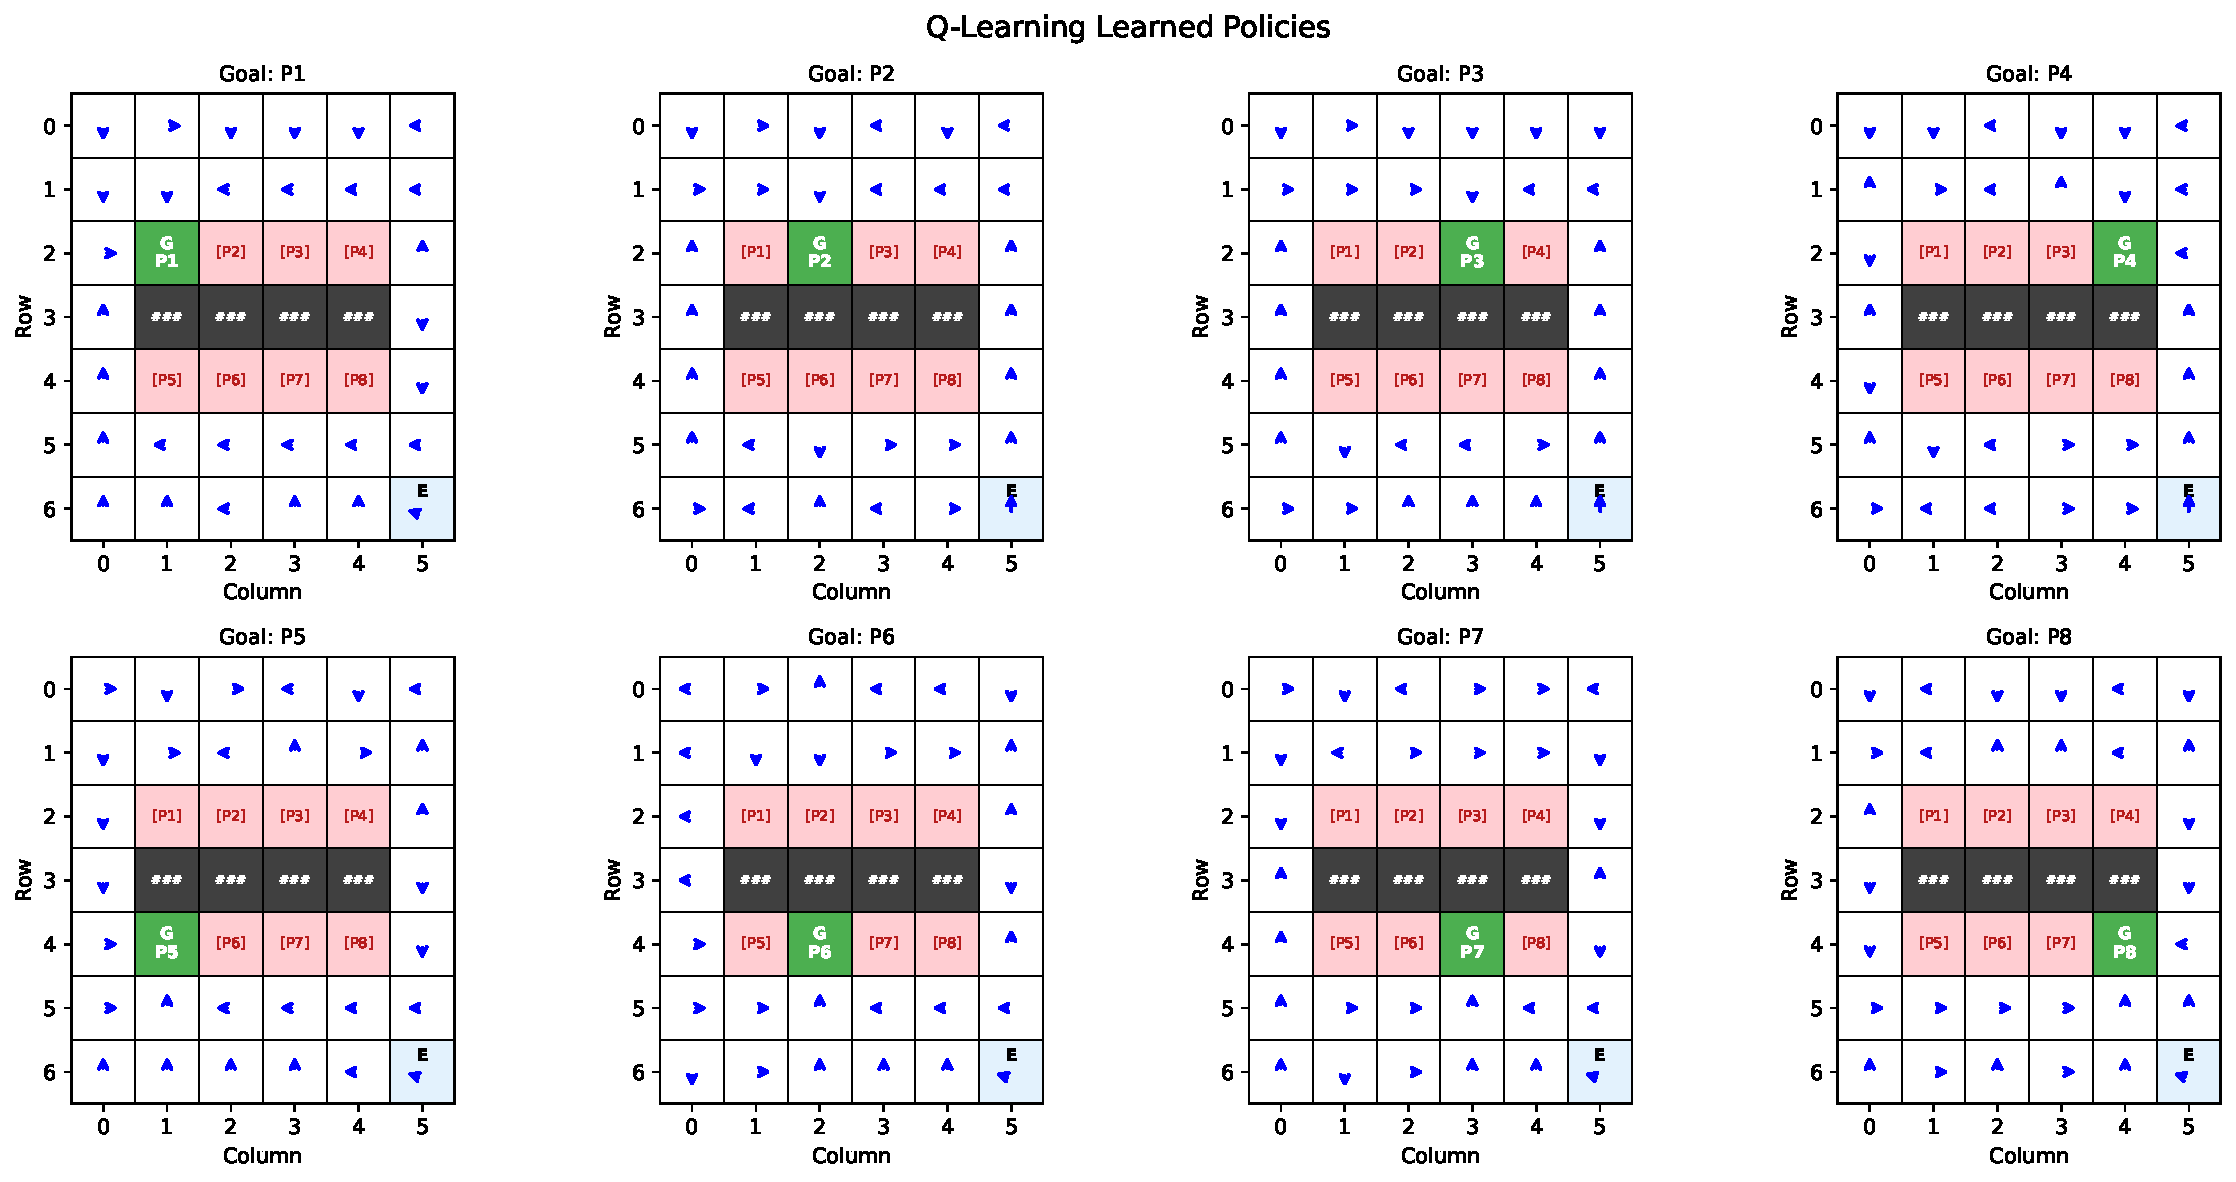
\includegraphics[width=0.95\columnwidth]{q_learning_policies.pdf}
    \caption{Q-learning policies for all 8 parking spots. Blue arrows indicate the greedy action at each walkable cell.}
    \label{fig:qpolicies}
\end{figure}

\textbf{Convergence comparison.} Figure~\ref{fig:convergence} compares the learning curves of Q-learning and DQN. Q-learning converges in approximately 1,500 episodes, while DQN requires approximately 3,000--6,000 episodes. This is expected---the $7 \times 6$ grid has only $\sim$29 walkable states per goal, which is well within tabular capacity. DQN's function approximation adds overhead (replay warm-up, target network lag, gradient noise) that is unnecessary at this scale but becomes essential for larger state spaces.

\begin{figure}[H]
    \centering
    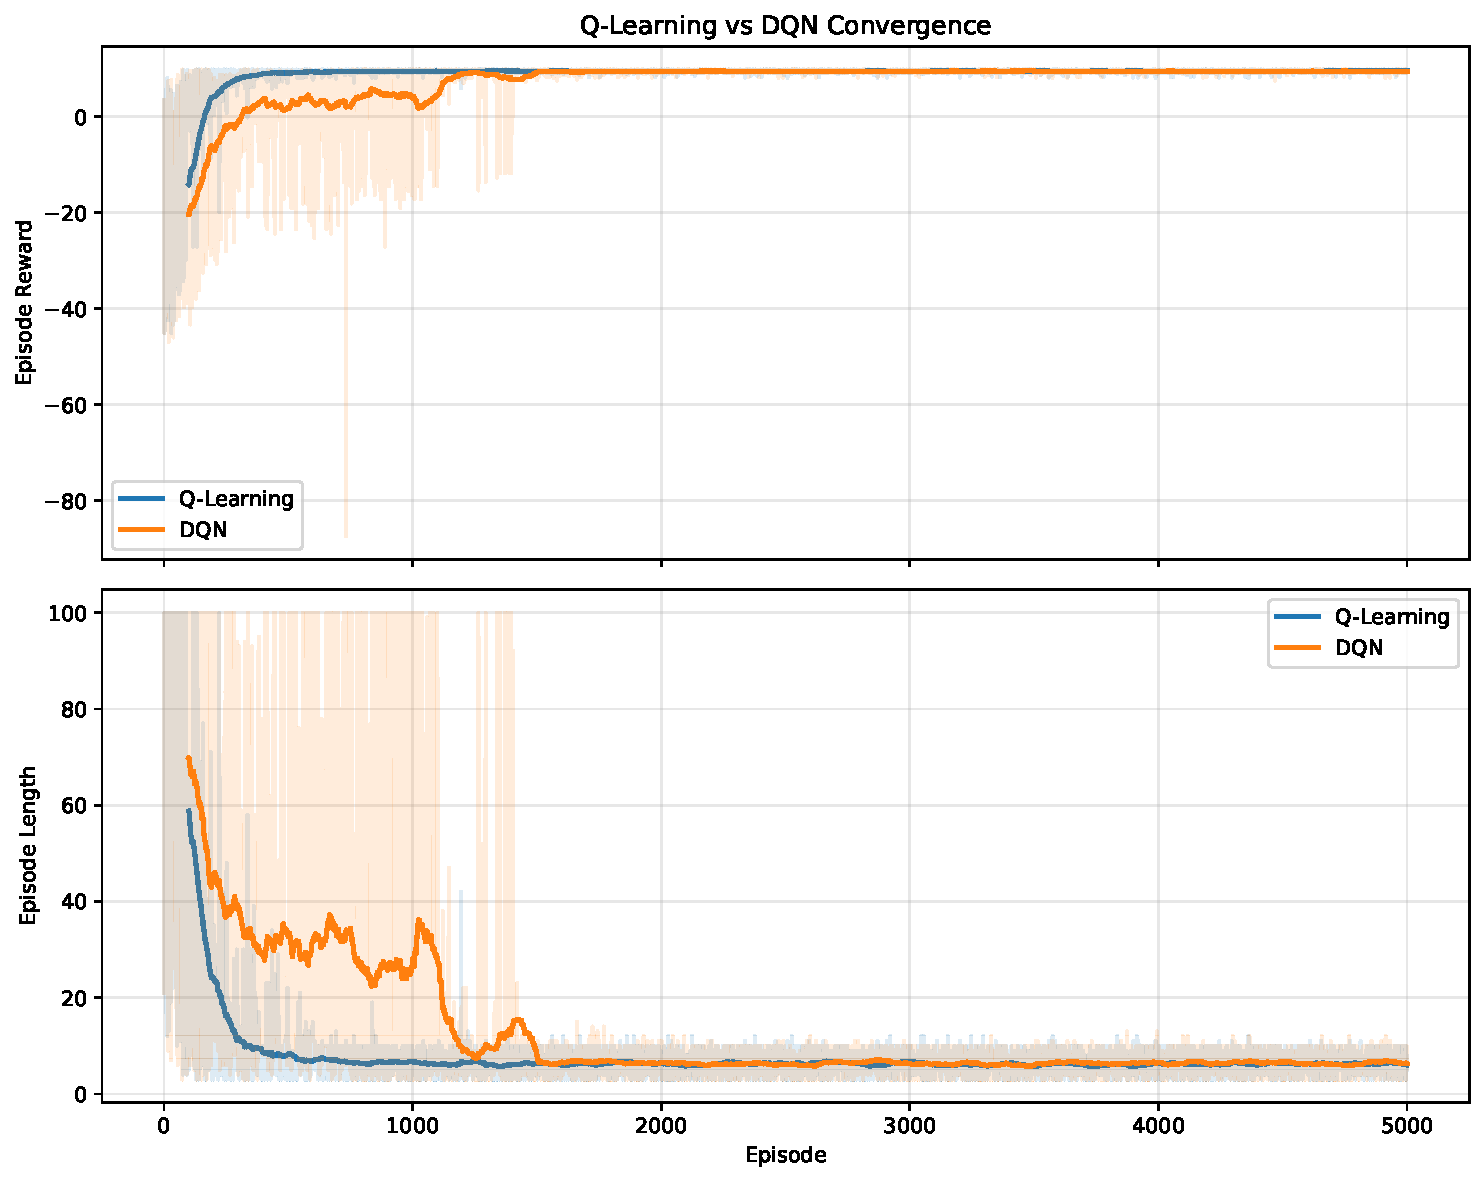
\includegraphics[width=0.95\columnwidth]{dqn_vs_tabular.pdf}
    \caption{Convergence comparison. Q-learning (blue) converges faster than DQN (orange) on the $7 \times 6$ grid. Moving average window = 100 episodes.}
    \label{fig:convergence}
\end{figure}

\textbf{Parameter sensitivity.} Figure~\ref{fig:params} shows how Q-learning convergence responds to changes in three key parameters.

\begin{figure}[H]
    \centering
    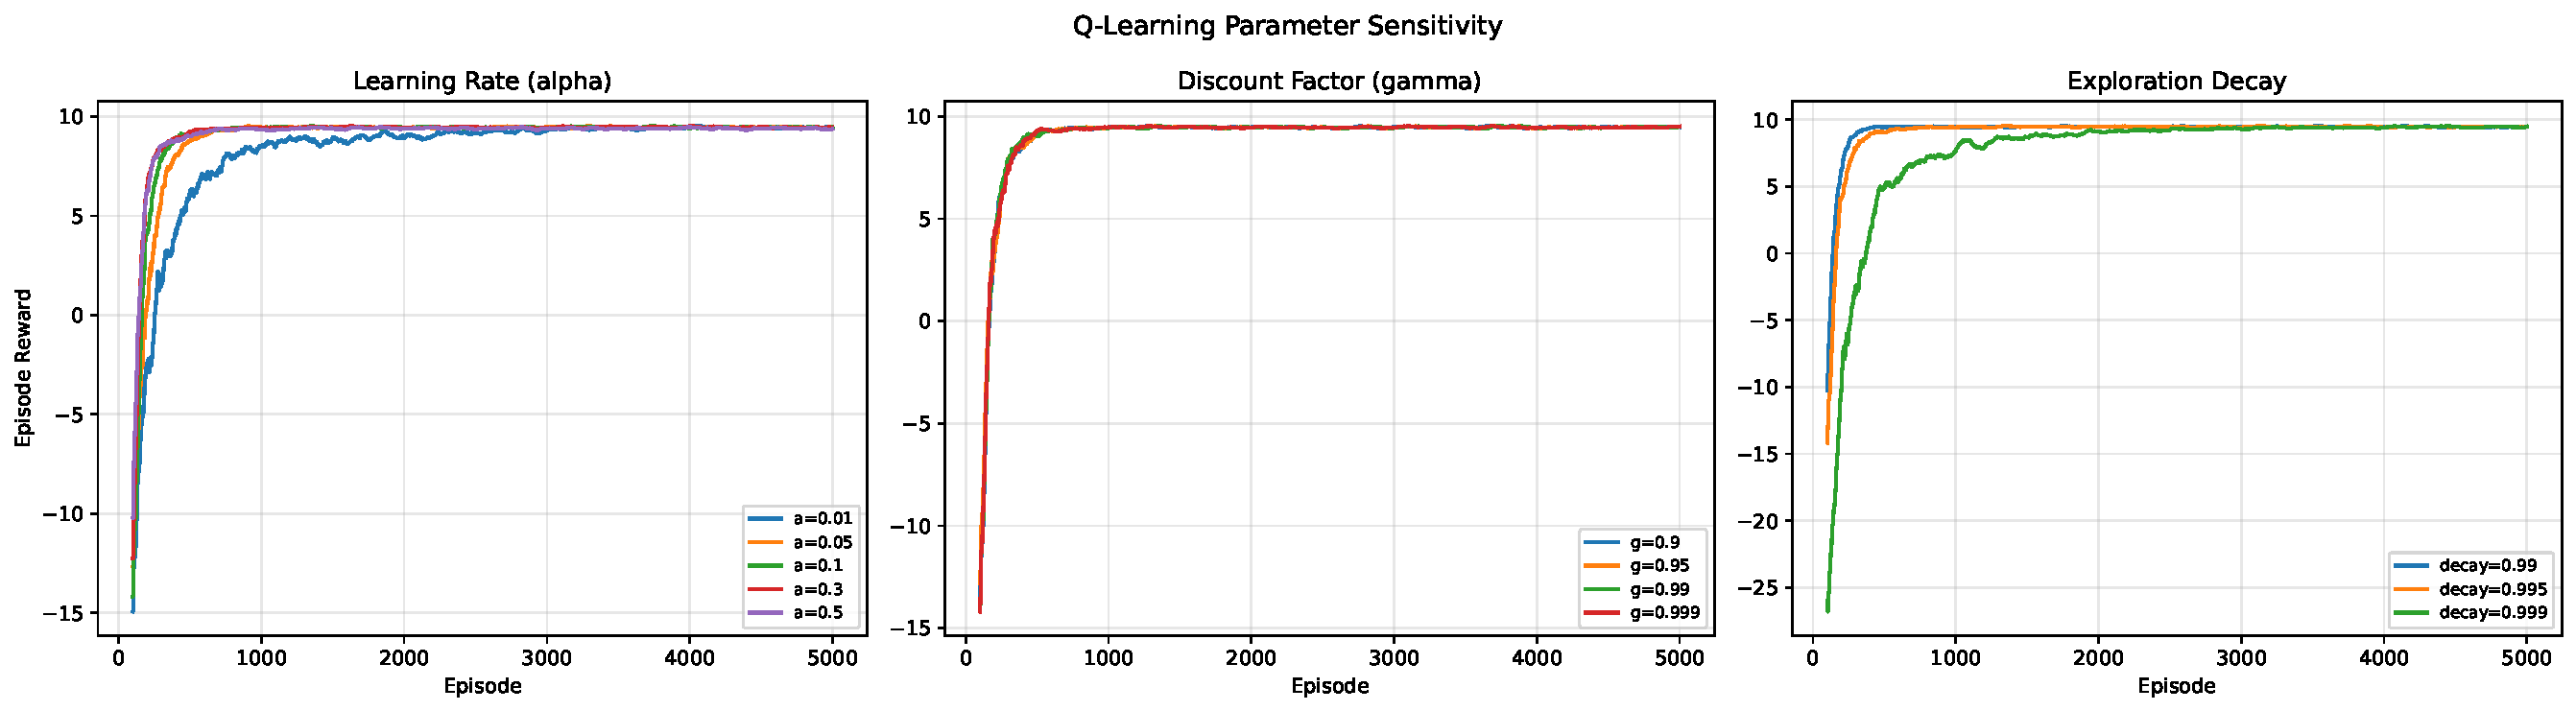
\includegraphics[width=0.95\columnwidth]{tabular_param_sensitivity.pdf}
    \caption{Q-learning parameter sensitivity. Left: learning rate $\alpha$. Center: discount factor $\gamma$. Right: exploration decay rate.}
    \label{fig:params}
\end{figure}

\textit{Learning rate} ($\alpha$): Values of 0.1 and 0.3 converge fastest. $\alpha = 0.01$ learns too slowly, while $\alpha = 0.5$ converges quickly but with higher variance in episode rewards.

\textit{Discount factor} ($\gamma$): All tested values (0.9, 0.95, 0.99, 0.999) produce optimal policies. However, $\gamma = 0.99$ provides the clearest value gradients toward distant goals. Lower discount factors undervalue long paths, which matters for spots like P1 that require 10 steps.

\textit{Exploration decay}: A decay of 0.99 converges earliest but risks insufficient exploration of the full state space. A decay of 0.999 explores more thoroughly at the cost of slower convergence. The default 0.995 balances the two.

\textbf{DQN multi-run reliability.} Figure~\ref{fig:multirun} shows DQN learning curves across 5 independent runs with different random seeds. All runs converge to optimal performance, with tight variance after approximately 4,000 episodes. This confirms DQN is not overly sensitive to initialization.

\begin{figure}[H]
    \centering
    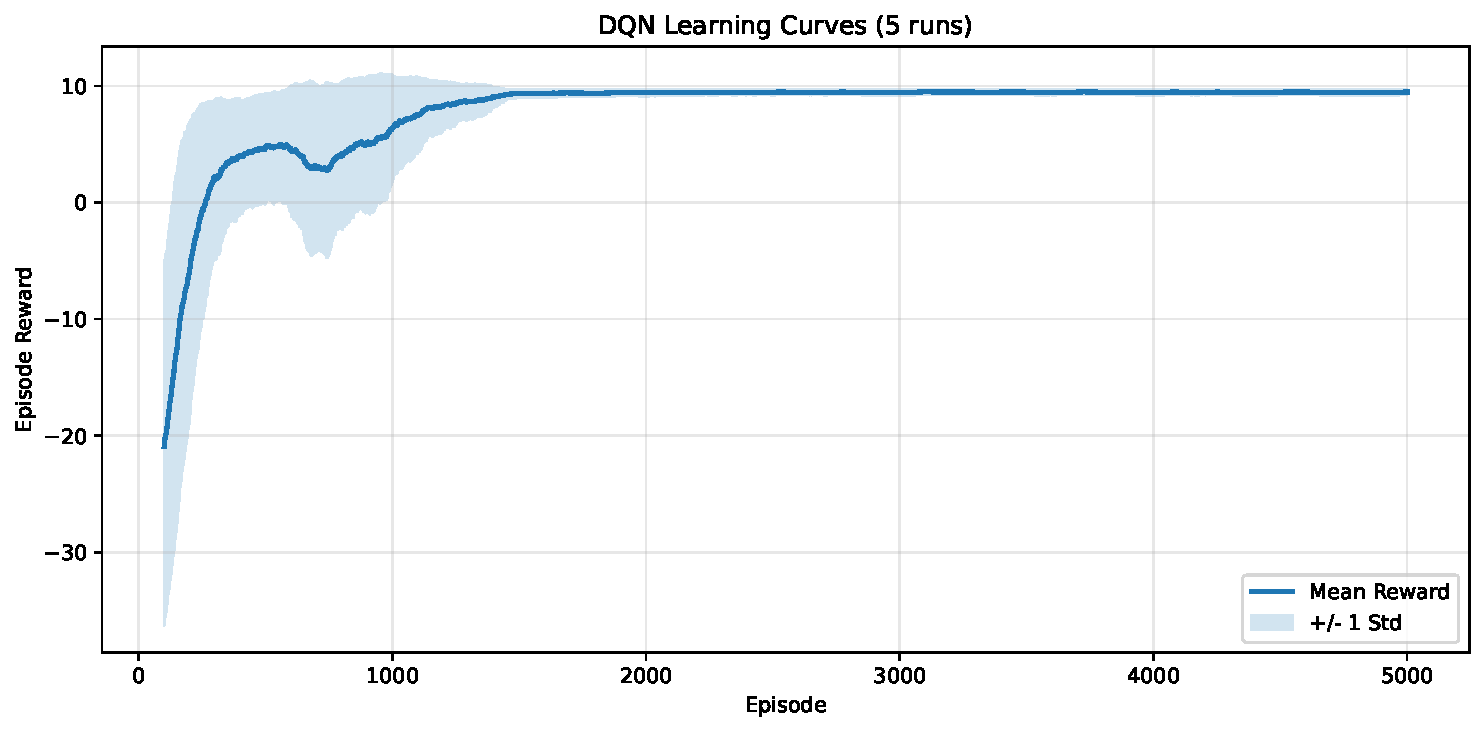
\includegraphics[width=0.95\columnwidth]{dqn_multi_run.pdf}
    \caption{DQN learning curves across 5 independent runs. Shaded region shows $\pm$1 standard deviation.}
    \label{fig:multirun}
\end{figure}


\subsection{Problem 2c: Enhancement --- Larger Parking Lot}

To test how the algorithms scale with complexity, we extended the environment to a $10 \times 12$ grid with 32 parking spots, up from the original 8. This increases the state space from 42 cells to 120 cells and quadruples the number of goals the agent must learn to reach.

\textbf{Layout generation.} The larger grid is generated procedurally using the same pattern as the base layout: two driving lanes at the top, then repeating blocks of parking row / barrier row / parking row, with a driving lane and entrance at the bottom. The barrier spans all columns except the rightmost, leaving a single passage on the right side. Parking spots are placed starting at column 1, centered within the available space.

\textbf{Training adjustments.} Episode counts were scaled linearly with the ratio of state-space sizes: $(10 \times 12) / (7 \times 6) \approx 2.86\times$. So tabular methods trained for approximately 14,300 episodes and DQN for approximately 8,600 episodes. No other hyperparameters were changed.

\textbf{Results.} Table~\ref{tab:scaling} compares the three algorithms on both grid sizes.

\begin{table}[H]
\centering
\caption{Scaling comparison: $7 \times 6$ (8 spots) vs.\ $10 \times 12$ (32 spots)}
\label{tab:scaling}
\begin{tabular}{@{}lcccc@{}}
\toprule
Grid & Method & Success & Avg Steps & BFS Avg \\
\midrule
$7 \times 6$ & Q-Learning    & 100\% & 6.3 & 6.3 \\
$7 \times 6$ & Double Q      & 100\% & 6.3 & 6.3 \\
$7 \times 6$ & DQN           & 100\% & 6.3 & 6.3 \\
\midrule
$10 \times 12$ & Q-Learning  & 100\% & 11.4 & 11.4 \\
$10 \times 12$ & Double Q    & 100\% & 11.4 & 11.4 \\
$10 \times 12$ & DQN         & 100\% & 11.4 & 11.4 \\
\bottomrule
\end{tabular}
\end{table}

All three algorithms achieve 100\% success with BFS-optimal paths on the larger grid. The tabular methods scale gracefully because they can represent each state independently---the Q-table simply grows from $\sim$1,300 entries to $\sim$15,400 entries. DQN's network does not grow at all; the same 17,540-parameter network handles both grids because it generalizes from the normalized position encoding. This is the practical advantage of function approximation: memory stays constant regardless of state-space size, while tabular memory grows linearly.

\textbf{Adaptations.} Two adaptations were made for the larger grid: (1) the maximum episode length was increased from 100 to 120 steps to accommodate longer paths, and (2) training episodes were scaled proportionally. No changes to the algorithms themselves, hyperparameters, or network architecture were required. This suggests the implementations are reasonably general.

\section{DreamerV3 on the Parking Lot}

DreamerV3 \citep{hafner2023dreamerv3} was trained on the same $7 \times 6$ parking lot to compare model-based reinforcement learning against the model-free methods described above. DreamerV3 is a model-based algorithm that learns a world model from image observations and trains its policy in ``imagination'' rather than through direct environment interaction.

\subsection{Environment Adaptation}

The parking lot was wrapped as a Gymnasium environment producing $64 \times 64$ RGB images. Six distinct colors encode the grid: dark gray for roads, medium gray for barriers, blue for non-goal parking spots, red for the goal spot, amber for the entrance, and green for the agent. The goal is communicated entirely through the image---the agent must learn that the red cell is the target.

\subsection{Training Configuration}

\begin{itemize}
    \item 100,000 environment steps with 4 parallel environments
    \item Train ratio 512 (512 dream steps per real environment step)
    \item Discount factor 0.99
    \item $64 \times 64$ image observations
    \item Evaluation every 5,000 steps (10 episodes per evaluation)
    \item Episode time limit: 100 steps
\end{itemize}

\subsection{Results}

DreamerV3 reaches near-optimal performance quickly---by step 22,500, eval return peaks at 9.7 (corresponding to $\sim$4 steps, near BFS-optimal for nearby goals). However, performance oscillates throughout training rather than converging to a stable policy. The full evaluation trajectory is shown in Table~\ref{tab:dreamer_qa}.

\begin{table}[H]
\centering
\caption{DreamerV3 evaluation returns (all 21 evaluations)}
\label{tab:dreamer_qa}
\begin{tabular}{@{}cccc@{}}
\toprule
Step & Return & Step & Return \\
\midrule
2,500   & $-65.3$ & 57,500  & $-6.0$ \\
7,500   & $-10.0$ & 62,500  & $+1.5$ \\
12,500  & $+1.8$  & 67,500  & $+5.7$ \\
17,500  & $-0.2$  & 72,500  & $+1.7$ \\
22,500  & $+9.7$  & 77,500  & $+9.4$ \\
27,500  & $+9.6$  & 82,500  & $+1.9$ \\
32,500  & $+5.8$  & 87,500  & $+5.5$ \\
37,500  & $+5.5$  & 92,500  & $+1.8$ \\
42,500  & $+9.4$  & 97,500  & $+1.5$ \\
47,500  & $+5.7$  & 102,500 & $+8.6$ \\
52,500  & $+1.8$  &         &        \\
\bottomrule
\end{tabular}
\end{table}

\textbf{Peak return:} $+9.7$ at step 22,500. \textbf{Last 5 average:} $+3.9$. Compare this to the model-free methods, which all achieve a stable $+9.1$ to $+9.8$ return after convergence.

\subsection{Analysis}

The returns cluster into three bands: near-optimal ($+8.6$ to $+9.7$, appearing 6 times), moderate ($+5.5$ to $+5.8$, appearing 5 times), and poor ($-0.2$ to $+1.9$, appearing 8 times). This suggests the agent solves nearby goals (P7, P8 with 3--4 BFS steps) reliably but struggles with distant goals (P1, P2 with 9--10 steps) that require longer navigation sequences around the barrier.

The core difficulty is representational. DreamerV3 receives the goal only as a colored pixel in the image. All 8 goals produce nearly identical images---the only difference is which of 8 small cells is red instead of blue. The tabular methods receive the goal ID as an explicit state variable, giving them unambiguous goal information. DreamerV3's world model must learn to distinguish which cell is red, associate that with different navigation strategies, and plan multi-step routes accordingly---all from a $64 \times 64$ image where the distinguishing feature occupies roughly 2\% of the pixels.

Model-based RL is designed for environments where real experience is expensive and imagination can substitute. The parking lot is the opposite: episodes are 3--10 steps, the state space has $\sim$29 walkable cells, and tabular methods exhaust the space in under 2,000 episodes. There is no advantage to building a world model when direct experience is this cheap.

\bibliography{references}

\end{document}
